\documentclass[border=3.14mm]{standalone}
\usepackage{pgfplots}
\pgfplotsset{compat=newest}

\begin{document}

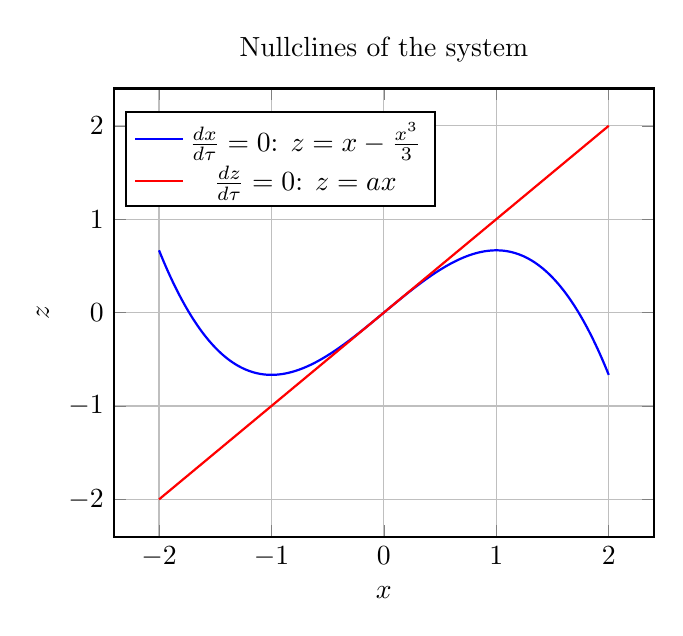
\begin{tikzpicture}
  \begin{axis}[
    domain=-2:2,
    samples=200,
    xlabel={$x$},
    ylabel={$z$},
    title={Nullclines of the system},
    legend style={at={(0.02,0.95)}, anchor=north west},
    grid=both,
    thick
  ]
    % dx/dτ = 0 nullcline
    \addplot[blue] {x - x^3 / 3};
    \addlegendentry{$\frac{dx}{d\tau}=0$: $z = x - \frac{x^3}{3}$}

    % dz/dτ = 0 nullcline, with parameter a
    \addplot[red, domain=-2:2] {1*x};  % a = 1
    \addlegendentry{$\frac{dz}{d\tau}=0$: $z = ax$}
  \end{axis}
\end{tikzpicture}

\end{document}
